%Plantilla Memoria T�cnica:
%Modificada por: Brenda Mariana Casillas Gonz�lez
%Última Modificación: 02-01-2023

%------------------------------CONFIGURACION DEL DOCUMENTO

\documentclass[12pt,letterpaper,spanish, xcolor=table]{report}
\usepackage[centertags]{amsmath}
\usepackage{amsfonts}
\usepackage{amssymb}	
\usepackage[utf8]{inputenc} % Usa solo esta línea
\usepackage{amsthm}
\usepackage[T1]{fontenc}
\usepackage{epsfig}
\usepackage{booktabs}
\usepackage{graphics}
\renewcommand{\baselinestretch}{1.5}
\renewcommand{\thefigure}{\thesection.\arabic{figure}}
\makeatletter
\@addtoreset{figure}{section}
\makeatother
\usepackage[spanish,activeacute]{babel}
\usepackage[numbers]{natbib}
\usepackage[hyphens]{url}
\usepackage{enumerate}
\usepackage{float}

\newenvironment{dedication}{\newpage\large\null\em\vskip1in}%
{\vfill}

\topmargin -1 in \oddsidemargin 0in \evensidemargin 0in
\textwidth 6.5in
\textheight 9in \pagestyle{myheadings}

% -----------------------------------INICIO DEL DOCUMENTO ---------------------------------------------------------------

\begin{document}
	
% Para la elaboraci�n de esta memoria t�cnica se debe usar un editor profesional que soporte Latex, como recomendaci�n se puede usar el WinEdt.

% El resultado que se sube a la plataforma debe ser en formato PDF

% Es importante mencionar que la redacci�n de este documento se debe hacer en tercera persona, cuidando escrupulosamente la ortograf�a, redacci�n y contenido, evitando el uso y abuso de adjetivos.
	
% ----------------------------------- CONTRAPORTADA -------------------------------------------------------------------------

%Se deben modificar los datos de la empresa, proyecto, asesores y alumnos
	
\thispagestyle{empty}

\begin{table}[ht]
  \centering
	\begin{tabular}{rr}
		\begin{minipage}[b]{0.05\linewidth}
		\hbox{
\psfig{file=Imagenes/logoUTZMG.jpg,height=1in,width=.8in}}
		\end{minipage}
	&
	\begin{minipage}[b]{.9\linewidth}
		\begin{center}
			\large{UNIVERSIDAD TECNOLÓGICA \\ DE LA ZONA METROPOLITANA DE GUADALAJARA}\\
		\end{center}
	\end{minipage}
	
	\end{tabular}%
\end{table}%

\begin{center}
	
\large{\textbf{MEMORIA TÉCNICA REALIZADA EN:}}
 \\ PiSA Farmacéutica

%%Logo de la empresa
\centerline{\hbox{
\psfig{file=Imagenes/logoPISA.png,height=1.2in,width=3in}}}

\large{\textbf{PROYECTO:} Soluciones Informáticas para Unidades de Servicios Administrativos}

\vspace{0.1in}
\large{\textbf{PARA OBTENER EL GRADO DE:}}

\large{Ingeniería (ING) en:}
\vspace{0.05in}

\large{DESARROLLO Y GESTIÓN DE SOFTWARE}
\\
\large{PRESENTADO POR:}

Jessica Aguilar Valderrama %(Empezando con el nombre  y después apellidos)

Luis Manuel Gómez López %(Empezando con el nombre  y después apellidos)

\vspace{0.2in}

\begin{tabular}{cc}
	\vspace{0.2in}
	\textbf{ASESOR INDUSTRIAL} & \textbf{ASESOR ACADÉMICO} \\
	
	Ricardo Adolfo Pineda González & Mildred Green Gama\\
	\multicolumn{2}{c}{\textbf{COORDINADOR DE CARRERA}
	\vspace{0.2in}
	} \\
	
	\multicolumn{2}{c}{
			Lizbeth Noriega Gutiérrez }
	\end{tabular}
	
\end{center}
%\vspace{0.1in}
\begin{flushright}\small{ TLAJOMULCO DE ZUÑIGA, JALISCO, ABRIL DEL 2025} \end{flushright}

\newpage



% ------------------------------ PORTADA -----------------------------------------------------

%Se deben modificar los datos de la empresa, proyecto y alumnos



\thispagestyle{empty}


\begin{center}
	
 \begin{minipage}[b]{.9\linewidth}
	\begin{center}
		\vspace{0.2in}
		\large{UNIVERSIDAD TECNOLÓGICA DE LA ZONA \\METROPOLITANA DE GUADALAJARA}\\
		\large{DIRECCIÓN DE DESARROLLO Y GESTIÓN DE SOFTWARE}\\
	\end{center}
\end{minipage}
\vspace{0.3in}



\centerline{\hbox{
\psfig{file=Imagenes/logoUTZMG.jpg,height=2.2in,width=1.7in}}}

\LARGE{\textbf{\textsc{Path de Ayuda}} }

\vspace{0.3in}
\large{\textbf{MEMORIA TÉCNICA REALIZADA EN:}}
 \\ \textsc{PiSA Farmacéutica}
		
\vspace{0.2in}
\large{\textbf{PARA OBTENER EL GRADO DE:}}

\large{Ingeniería (ING) en:}

\large{DESARROLLO Y GESTIÓN DE SOFTWARE}
\\

\vspace{0.2in}
\large{PRESENTADO POR:}


\textsc{} Jessica Aguilar Valderrama %(Empezando con el nombre y despu�s apellidos)

\textsc{}Luis Manuel Gómez López

\vspace{0.3in}
\small{ ABRIL 2025}
\end{center}
%\vspace{0.1in}


\newpage


% -------------------------------------- DEDICATORIA ---------------------
% Esta secci�n es opcional, pero se recomienda que se ponga, se puede redactar hasta el final y tratar que no sea mayor a una cuartilla.

		\thispagestyle{empty}
		\addcontentsline{toc}{chapter}{Agradecimientos}
		
		\begin{dedication}
			Agradezco a todas las personas ....
		\end{dedication}


%-------------------------------- �NDICE


\tableofcontents


% --------------------------------------- CAP�TULOS DEL DOCUMENTO ----------------------------------------
% ____________________________________________________________________________________


\pagenumbering{arabic}
\oddsidemargin 0.2in \textwidth 6.5in \topmargin -0.25in
\textheight 9in \pagestyle{myheadings}
	
	
\newpage

% CAPITULO INTRODUCCI�N. Enmarca y situa el trabajo a realizar. Tiene por objeto proporcionar una visi�n general del documento.
%____________________________________________________________________________________________________________________


\chapter{Introducción}
\newpage




% CAPITULO ANTECEDENTES Y DESCIPCI�N DE LA EMPRESA. Tiene por objeto proporcionar una visi�n general del documento.
%____________________________________________________________________________________________________________________
\chapter{Antecedentes y Descripción de la Empresa}
\newpage


%Nota: Los puntos que siguen son una propuesta, pongan solo los puntos que apliquen en su empresa y que los permitan poner, tambi�n puede agregar otros puntos si lo cree conveniente.

\section{Ubicación}
	
\begin{figure}[htp]
	\centering
	Av España 1802, Moderna, 44190 Guadalajara, Jal.
	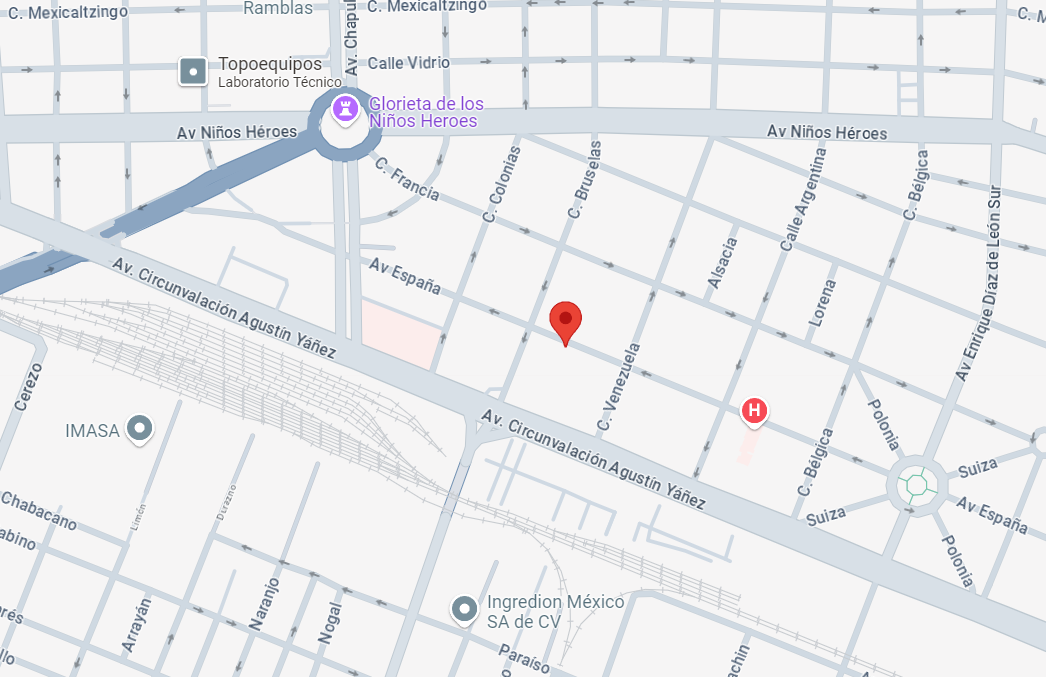
\includegraphics[width=0.8\textwidth]{Imagenes/ubicacion.png}
	\caption{Mapa ubicación Laboratoriso PiSA S.A DE C.V}\label{a1}
\end{figure}


% Poner la direcci�n y un mapa que puede salir de maps.google.com


\section{Misión}
Somos un Grupo de Empresas Responsables, confiables, éticas, con vocación de servicio; comprometidas con sus colaboradores y la salud.

\section{Visión}
Permanencia a través de innovación y crecimiento acelerado en México y en el extranjero.
	
\section{Organigrama}

\begin{figure}[H]
	\centering
	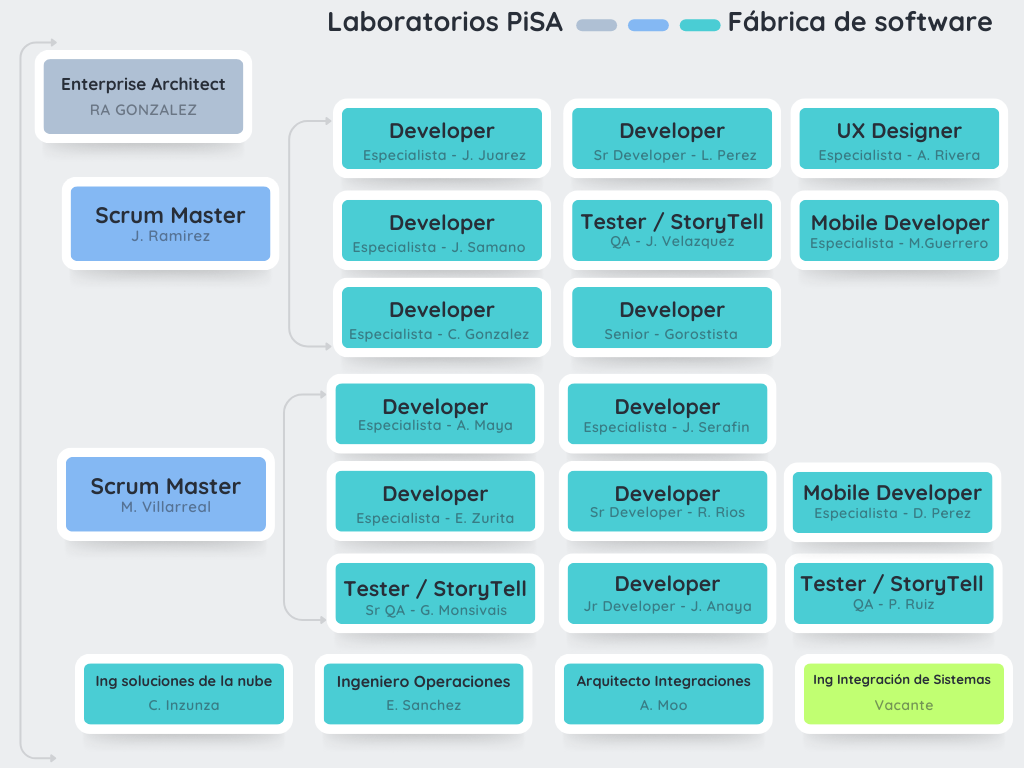
\includegraphics[width=0.9\textwidth]{Imagenes/OrganigramaPisa.png}
	\caption{Organigrama de Fábrica de Software}\label{a1}
\end{figure}
	
\section{Giro de la empresa}

PiSA Farmacéutica es una empresa dedicada a la fabricación, comercialización y distribución de medicamentos y dispositivos médicos en el tratamiento de un amplio ramo de la salud

\section{Historia}

PiSA Farmacéutica es una empresa mexicana, con 77 años de historia, desarrollando productos y servicios integrales para los segmentos de salud pública y privada en México, Estados Unidos, Latinoamérica y el Caribe.

\newpage
% -------------------------------- CAPITULO PROBLEM�TICA --------------------------------------
%____________________________________________________________________________________________________________________
	
\chapter{Problemática y Descripción del Proyecto}
\newpage

% En esta secci�n se deber� redactar un planteamiento de la problem�tica que se pretende resolver.
\section{Problemática}

	En el desarrollo de software, una administración de proyectos eficiente es clave para garantizar calidad y cumplimiento de objetivos. Sin embargo, la falta de documentación técnica bien estructurada dificulta la comprensión del proyecto y afecta el trabajo de equipo provoca que esta documentación sea inconsistente, incompleta o desactualizada, lo que dificulta la realización de pruebas precisas y la identificación temprana de errores. \\
	
	La ausencia de una documentación clara y bien definida genera problemas en la comunicación entre los diferentes equipos de trabajo, dificultando la alineación de objetivos y la comprensión de los requerimientos del sistema. Esto impacta negativamente en la calidad del producto final, ya que se incrementan los riesgos de malinterpretaciones, modificaciones no documentadas y errores en la implementación.
	

%Escribir un resumen de su proyecto en donde se hable del aspecto económico, operativo, técnico, humano, objetivos, etc.
\section{Descripción del Proyecto}
	
	Desarrollar un enfoque estructurado para la elaboración de documentación técnica en proyectos de software, asegurando que sirva como una herramienta clave para la administración eficiente del desarrollo. Esta documentación permitirá mejorar la comunicación entre los equipos, optimizar la gestión de requisitos y garantizar que el software cumpla con los estándares de calidad y las expectativas del usuario final.


%Describir cual es el objetivo general que persigue el proyecto.
\subsection{Objetivo General}

	Se enfocará en la creación de guías, plantillas y metodologías que permitan documentar de manera clara los requerimientos, la arquitectura y los criterios de aceptación del software. Se trabajará en conjunto con el equipo de Quality Assurance (QA) para garantizar que la documentación cumpla con los estándares de calidad necesarios para la ejecución eficiente de pruebas y validaciones.\\
	
	Reduciendo el riesgo de errores y mejorando la trazabilidad del proyecto. Con ello, se busca optimizar la administración del proyecto, reducir tiempos de desarrollo y asegurar que el producto final cumpla con las expectativas del usuario y los estándares de la industria.\\
	
	Esta documentación facilitará la comprensión del sistema, mejorará la comunicación entre equipos y permitirá una mejor gestión de cambios, optimizando el proceso de desarrollo.
	


%Describir cuales son los objetivos específicos que persigue el proyecto. Mínimo deben ser dos y estos deben abonar al objetivo general
\subsection{Objetivos Específicos}

	1. Establecer lineamientos para la estructuración de documentos que faciliten la gestión de requisitos y planificación del desarrollo.\\
	
	2. Mejorar la comunicación entre los equipos de trabajo mediante documentación clara y organizada.\\
	
	3. Reducir el riesgo de errores en el desarrollo a través de documentación detallada y bien estructurada.\\
	
	4. Garantizar que la documentación técnica cumpla con estándares de calidad y facilite la trazabilidad del proyecto.\\
	
	5. Apoyar al equipo de Quality Assurance (QA) en la elaboración de documentación que permita validar el cumplimiento de los requisitos del software.\\

	
	
%Describir de manera detallada las actividades para el desarrollo de la estadía y/o proyecto (Diagrama de Gantt).
\subsection{Planeación}



%CAPITULO MARCO TEÓRICO: bases teorícas del proyecto. conceptos básicos y antecedentes o información existente.
%____________________________________________________________________________________________________________________
	
\chapter{Marco Teórico}
\newpage

La administración de proyectos de software es un proceso que integra metodologías y técnicas para la planificación, programación, ejecución y seguimiento de proyectos de desarrollo. Su principal objetivo es optimizar el trabajo de los desarrolladores mediante una adecuada gestión de recursos, garantizando que el proyecto se lleve a cabo de manera eficiente y productiva. Además, permite minimizar los riesgos asociados y responder de manera efectiva ante cualquier dificultad que pueda surgir en el proceso de desarrollo (Tiffin University, 2024). \\

Dentro de la administración de proyectos, la planificación juega un papel fundamental, ya que define el rumbo del proyecto desde su concepción hasta su finalización. En esta fase, se establecen los alcances, se asignan los recursos necesarios, se diseña un cronograma de ejecución y se implementan estrategias de comunicación. Asimismo, se consideran elementos clave como las pruebas y el mantenimiento del software, garantizando su correcto funcionamiento y su sostenibilidad a lo largo del tiempo (Wrike, 2024).\\

Otro aspecto esencial en el desarrollo de software es la documentación, pues permite estructurar y registrar la información clave del proyecto. A pesar de su importancia, en muchas ocasiones es percibida como una tarea que resta tiempo productivo. Sin embargo, la ausencia de documentación adecuada puede dificultar la comprensión del sistema, limitar su escalabilidad y complicar su mantenimiento a largo plazo. La documentación puede incluir especificaciones funcionales, diagramas de casos de uso y mockups de interfaces, entre otros elementos que faciliten el desarrollo y la futura gestión del software (Arsys, 2024).\\

La gestión de requisitos es otro pilar clave en la administración de proyectos de software, ya que permite definir, analizar, priorizar y validar las necesidades del sistema. Para ello, se elabora un Plan de Gestión de Requisitos (RMP), el cual establece los procesos de recopilación, documentación y control de requisitos a lo largo del ciclo de vida del proyecto. Este enfoque permite garantizar que el producto final cumpla con las expectativas del cliente y los estándares de calidad, al tiempo que facilita la detección temprana de errores y contribuye a la reducción de costos y riesgos (IBM, 2024).\\

Además de la planificación y gestión de requisitos, el Análisis de Puntos de Función (FPA, por sus siglas en inglés) se ha convertido en una herramienta fundamental en la medición de la funcionalidad de un sistema de software. Este enfoque permite cuantificar el tamaño de un proyecto con base en elementos como datos procesados, tipos de transacciones y consultas realizadas. A partir de esta información, los desarrolladores pueden identificar áreas que requieren optimización y realizar análisis comparativos de rendimiento con relación a estándares de la industria (BlueOptima, 2024).\\

El FPA también resulta útil para estimar el tiempo y los recursos necesarios en el desarrollo de un proyecto, lo que facilita una planificación más precisa y una gestión más eficiente del proceso. Su aplicación permite evaluar la productividad del equipo, monitorear el progreso del proyecto y mejorar el análisis de costo-beneficio, asegurando que las decisiones sobre inversiones y asignación de recursos se tomen de manera fundamentada. Además, contribuye a alinear los esfuerzos de desarrollo con los objetivos estratégicos de la organización, garantizando que el software desarrollado genere valor a los usuarios finales (GeeksForGeeks, 2024).\\


Las pruebas de software son un proceso esencial en el desarrollo de aplicaciones, cuyo objetivo principal es evaluar su funcionalidad e identificar posibles errores antes de su implementación final. Según Certus (2022), << este proceso garantiza que el software cumpla con los estándares de calidad y que el producto entregado sea confiable y eficiente>>.\\

En la industria del software, el aseguramiento de calidad (QA) y las pruebas forman una parte crucial del ciclo de vida del desarrollo de software (SDLC). IBM (2023) señala que defectos en el software pueden dañar la reputación de una empresa, frustrar a los clientes e incluso generar pérdidas económicas significativas. Por ello, el control de calidad es indispensable para evitar retrasos en las entregas y garantizar el funcionamiento óptico de los sistemas.\\

El control de calidad en el desarrollo de software se implementa a través de un procedimiento metódico que supervisa y revisa cada etapa del desarrollo. BrowerStack (2023) destaca que este proceso incluye actividades como análisis de requisitos, preparación de pruebas, ejecución de pruebas, seguimiento de defectos y redacción de informes.\\

IBM (2023) resalta que la tendencia actual en la industria es realizar pruebas continuas, es decir, iniciar las pruebas desde la fase de diseño, continuar con ellas durante el desarrollo y mantenerlas incluso en producción. Este enfoque permite detectar errores con mayor anticipación y mejorar la calidad del producto final.\\

Para logar una validación integral del software, es fundamental definir correctamente los escenarios y casos de prueba. Leapwork (2025) los describe de la siguiente manera
Los escenarios de prueba es un documento de alto nivel que describe la funcionalidad que se evaluará, proporcionando una visión general de lo que debe probarse. Se centra en el comportamiento de software sin entrar en detalles específicos.\\

Los casos de prueba son un conjunto de condiciones o variables específicas que permiten evaluar si un sistema cumple con los requisitos establecidos. Incluyendo entradas, condiciones, procedimiento y resultados esperado, guiando al evaluador paso a paso.\\

La correcta implementación de estos elementos permite asegurar el correcto funcionamiento del software en diversas situaciones y garantizar un producto de alta calidad. Como afirma IBM (2023), las pruebas continuas y bien estructuradas contribuyen a minimizar riesgos y mejorar la satisfacción del usuario final, optimizando el rendimiento de las aplicaciones en un mercado altamente competitivo.\\




%CAPITULO DESARROLLO DEL PROYECTO: procedimiento o descripci�n de las actividades realizadas, como es un desarrollo es importante
%____________________________________________________________________________________________________________________


\chapter{Desarrollo del Proyecto}
\newpage
	
\section{Path de ayuda}

\subsection{Levantamiento de requerimeintos}

\subsection{Descripcion de requerimeintos}

\subsection{FPs}

\subsection{Casos de prueba}



\section{Calculadora Nutricional}

\subsection{Levantamiento de requerimientos}

\subsection{Casos de prueba}













	




	
\section{Análisis y Diseño}

\section{Implementación}

\section{Pruebas}


% CAPITULO RESULTADOS(estatus del proyecto y posibles mejoras) Y CONCLUSIONES(problemas presentados, costos, restrasos, cumplimiento de objetivos, etc)
%____________________________________________________________________________________________________________________
	
	
\chapter{Resultados y Conclusiones}
\newpage
	
\section{Resultados}

\section{Conclusiones}


% -------------------------- ANEXOS
%____________________________________________________________________________________________________________________
	

\newpage
% APENDICE O ANEXO (infoemacion adicional que se quiera anexar o agregar
% BIBLIOGRAFIA
\appendix
	
%\chapter{Bibliograf\check{}�a}
%\bibliographystyle{apalike}
\bibliographystyle{unsrtnat}
	
	
\begin{itemize}
	\item A
	\item B
	\item C
\end{itemize}



\newpage
\chapter{Bibliografía}

	Intel. (n.d.). \textit{Descripción general y ejemplos de los sistemas en tiempo real}. Intel. Recuperado de {https://www.intel.la/content/www/xl/es/robotics/real-time-systems.html}\\
	
	IBM. (2023, diciembre 20). \textit{Monitoreo de condiciones. ¿Qué es el monitoreo de condiciones?} Recuperado de {https://www.ibm.com/mx-es/topics/condition-monitoring}\\
	
	Latam, T. (2023, junio 8). \textit{Gestión de la producción: qué es, etapas y cómo hacerlo}. TOTVS. Recuperado de {https://es.totvs.com/blog/gestion-industrial/gestion-de-la-produccion-que-es-etapas-y-como-hacerlo/}\\
	
	Katana. (2024, mayo 22). \textit{Production Management Software for Manufacturers — Katana}. Recuperado de {https://katanamrp.com/production-management-software/}\\
	
	Admin. (2023, febrero 12). \textit{La automatización industrial: ¿Qué es? Sus características más relevantes}. AUTEXOPEN. Recuperado de {https://www.autex-open.com/automatizacion-industrial/automatizacion-industrial/}\\
	
	SafetyCulture. (2024, enero 15). \textit{Sistema Andon: Cómo funciona el sistema}. Recuperado de {https://safetyculture.com/es/temas/sistema-andon/}\\
	
	Mapex. (2024, julio 1). \textit{¿Qué es el sistema Andon y cuáles son sus beneficios?} Recuperado de {https://mapex.io/news/sistema-andon-definicion-y-beneficios/}\\
	
	Romero, P. (2022, diciembre 7). \textit{¿Qué es Andon? Sistema de control visual de producción}. Geinfor ERP. Recuperado de {https://geinfor.com/que-es-andon-sistema-de-control-visual-de-produccion/}\\
	
	Galiana, P. (2024, abril 9). \textit{GUÍA: ¿Qué es SAP y qué soluciones ofrece?} Thinking for Innovation. Recuperado de {https://www.iebschool.com/blog/que-es-para-que-sirve-sap-management/}\\
	
	Hiberus. (2024, enero 25). \textit{¿Qué es SAP y para qué sirve?} Blog de Hiberus. Recuperado de {https://www.hiberus.com/crecemos-contigo/que-es-sap/}\\
	
	SAP. (s.f.). \textit{¿Qué es SAP? Definición y significado}. Recuperado de {https://www.sap.com/latinamerica/about/what-is-sap.html}\\
	
	Certus. (2022, abril 13). \textit{Las pruebas de software y su importancia}. Certus Blog. Recuperado de {https://www.certus.edu.pe/blog/pruebas-de-software-importancia/}\\
	
	IBM. (2024, mayo 9). \textit{¿Qué son las pruebas de software y cómo funcionan?} Recuperado de {https://www.ibm.com/mx-es/topics/software-testing}\\
	
	Roy, S. (2023, junio 21). \textit{Quality Assurance vs Testing}. BrowserStack. Recuperado de {https://www.browserstack.com/guide/quality-assurance-vs-testing}\\
	
	Schwartz, C. (2025, enero 30). \textit{Test Cases vs Test Scenarios: Definition, Examples and Template}. Leapwork. Recuperado de {https://www.leapwork.com/blog/test-case-vs-test-scenario}\\
	
	Mapex. (2023, septiembre 15). \textit{Tecnología móvil: ¿cuál es su potencial en las empresas industriales?} Recuperado de {https://mapex.io/news/tecnologia-movil-empresas-industriales/}\\
	
	Toobler. (s.f.). \textit{Industry-Specific Web Application Development Guide - 2025}. Recuperado de {https://www.toobler.com/blog/industry-specific-web-application-development}\\
	
	Afzal, M. (2024, julio 8). \textit{Cross browser compatibility - web apps that work universally}. LambdaTest. Recuperado de {https://www.lambdatest.com/learning-hub/cross-browser-compatibility}\\
	
	AppMaster. (s.f.). \textit{Compatibilidad con dispositivos móviles}. Recuperado de {https://appmaster.io/es/glossary/compatibilidad-con-dispositivos-moviles}\\
	


\newpage	
\chapter{Glosario}

\begin{description}
	\item[Asesor Acadámico] Persona encargada de regañar a los alumnos
\end{description}
	
%Otro apendice

\end{document} 
